\chapter{Interpreting the output}   \label{cap:analysis}
\lettrine{T}he outputs of EpiGrass simulations were designed to be as flexible as possible. Beside the automated report generation which serves as an overview of the model and its results, raw data is also made available for ready utilization from other softwares such as R and Grass.

\section{Visualization}

On the graphical user interface, if you check the box \texttt{Visualize Graph}, a 3D display opens up when the simulation is started. This display will plot the network on the map (if a map is available). As the simulation progresses, the nodes  change color from green to red as the localities become infected. Localities that get infected later are assigned a different shades of red which will tend to become blue as the time progresses. This way the sequence of infection remains visible throughout the simulation by means of this color scale.

The visualization module can also be invoked independently of the simulation to review the dynamics of simulation data stored on the database. This way, any previous simulation can be reviewed at any time. It is also recommended that simulataneous visualization be turned off to speed up calculations.  

Currently, the visualization module displays only the temporal dynamics of infection with the number of infected individuals in each infected locality is represented by the size of the node object in the network plot. 

\section{Database}
The simulated time series are stored in a MySQL table in the database epigrass: E, I, S, incidence (L), together with time, geocode and coordinates. The table is named after the filename of the script and date and time of the simulation.

Epigrass provides an R script for importing the data into R for further analysis and display \footnote{see appendix \ref{cap:introR}}.     

\section{Epidemiological descriptors}
At the end of the simulation, Epigrass calculates a set of epidemiological stats. These stats are presented to the user in two ways: as a .csv table that can be imported by R or any other statistical package; and as a written (PDF format) report.  Stats include descriptors of the epidemic dynamics at the whole graph level and also node-specific stats:
\paragraph*{Graph-level stats:}
\begin{description}
\item[Epidemic pop size] Total number of cases in the whole graph during the simulation. 
\item[Epidemic size] Total number of cities that had authoctonous transmission during the simulation. 
\item[Mean epidemic speed] Average number of new localities infected per time step.
\item[Epidemic Duration] Time between the first and last case.
\item[Median survival] Time to reach 50\% of the cities.
\item[Vaccinated] Total number of vaccinated individuals.
\item[Quarantined] Total number of quarantined individuals.
\item[Pass] Total number of infected individuals travelling through the network.
\item[Top ten nodes] Main cities in terms of number of infected.
\item[First ten nodes] First ten infected cities.
\end{description}

At the site scale, the report returns for each site $i$:
\begin{description}
\item[Incidence] Accumulated number of new cases per time step
\item[Local epidemic size] Total number of cases that occurred in the site during the simulation.
\item[Infectious arriving] Number of infected individuals arriving per time step


%\item[Local outbreak start point($t_i$)] Time step of first authoctonously transmitted infection in $i$.
%\item[Local arrival ($y_i$)] Total number of infected individuals that visited $i$ during the simulation.
%\item[Speed of spread($\sigma_1$)] Number (or proportion) of new localities infected per time step
%\item[Speed of spread($\sigma_2$)] Number (or proportion) of new localities infected per time step, weighed by population size of these localities (?).
%\item[Speed of propagation($\sigma_3$)] Velocitity of propagation in $km^2/day$, where velocity of propagation is defined as a velocity $c$ so that, if you run faster than $c$, you leave the epidemi behind and, if you run slower than $c$, the epidemic will eventually surrounds you (Rass and Radcliff. Spatial Deterministic epidemics, livro).
%\item[Speed of propagation($\sigma_4$)] Velocity of movement of the centroid of the epidemic region.
%\item{Mean direction of spread}
%\item{}   
\end{description}

\section{Network Descriptive Statistics}
EpiGrass automatically calculates and displays descriptive statistics about the network structure in Reports 1 and 3.
\subsection{Basic Numbers}
       \begin{description}
        \item[Order (Number of Nodes):] The Number of localities the network is composed of.
        \item[Size (Number of Edges):] The number of transportation routes connecting any pair of nodes. 
	\item [Eulerian:] Can be yes or No depending on if the networkgrap is eulerian o not. A Eulerian graph contains a circuit (Eulerian circuit) which includes all nodes an edges of the graph.
	\item [Traversable:]Can be Yes or No depending on if the network graph contains an Eulerian trail, i.e. a trail tht includes all the nodes an edges of the graph.   
        \end{description}
        
	\subsection{Shortest-path Distribution}
	In a network there are frequently more than one path from locality A to locality B. Of these possible  routes, the shortest path is the most important when dealing with epidemic processes over networks.
	
        A network distance Matrix can be calculated whose elements represent the number of edges separating any pair of nodes via the shortest path between them. From this matrix a histogram of the Shortest-paths lengths can be generated which gives us an idea of give us an idea of how fast an epidemic would spread in our network, if distance was the only factor.
        
        
        \subsection{Conectivity Matrix}
        The most basic measure of accessibility involves network connectivity
        where a network is represented as a connectivity matrix(figure \ref{fig:cm}), which 
        expresses the connectivity of each node with its adjacent nodes. 
        
        The number of columns and rows in this matrix is equal to the number 
        of nodes in the network and a value of 1 is given to each cell representing a directly connected pair and a value of 0 to each cell representing an unconnected pair. The summation of this matrix, along its rows or collumns, provides a very 
        basic measure of node accessibility, also known as the degree of a node.
        \begin{figure}[h]
        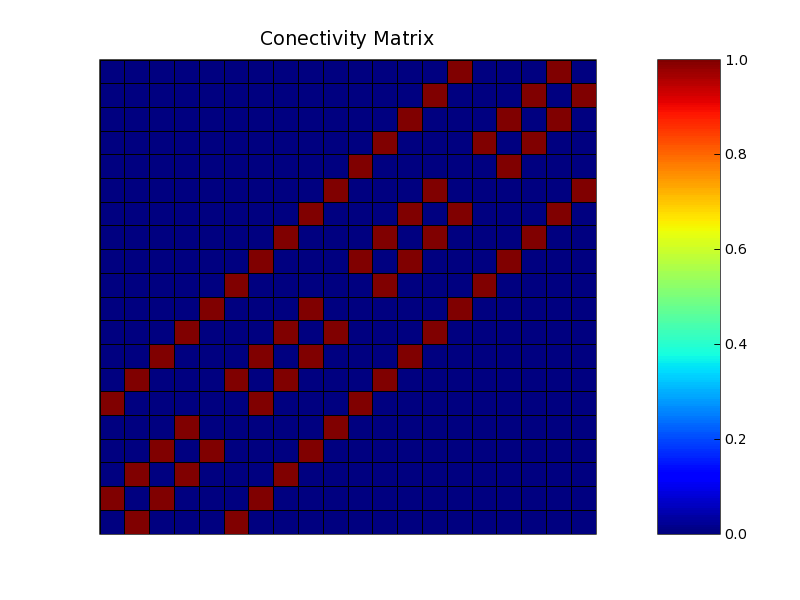
\includegraphics[scale=0.6]{cm.png}
        \centering
        \caption{Connectivity matrix of a simple grid network}
        \label{fig:cm}
        \end{figure}
        
        indices = r"""
        \subsection{Number of Cycles}
	A cycle is a circular path, meaning that in ends wher it started, that does not repeat an edge. The index presented here is the maximum number of independent cycles in a network.
	
        This number ($u$) is estimated by knowing the number of nodes ($v$), 
        links ($e$) and of sub-graphs ($p$);
        
        Trees and simple networks will have a value of 0 since they have 
        no cycles. 
        The more complex a network is, the higher the value of u, 
        so it can be used as an indicator of the level of development 
        of a transport system.
        
        $$ u=e-v+p$$
        
        \subsection{Wiener Distance}
        The Wiener distance is the sum of all the shortest distances in the network.
        
        $$D_W =\sum_{i=1}^v\sum_{j=1}^i\;D_{ij}$$
	
	where $D$ is the Shortest distance matrix.
        
        \subsection{Mean Distance}
        The mean distance of a network is the mean of of the set of shortest paths, 
        excluding the 0-length paths.
        
        $$\bar{D}=\frac{1}{v}\sum_{i=1}^v\sum_{j=1}^i\;D_{ij}\;\;\; \forall\; D_{ij}\neq0$$ 
        \subsection{Network Diameter}
        The diameter of a network is the longest element of the shortest paths set.
        
        \subsection{Length of the Network}
        The length of a network is the sum in metric units (e.g., km) of all the edges in the network.

        \subsection{Weight of the Network}
        The weight of a network is the weight of all nodes in the graph ($W(N)$), which is the summation 
        of each node's order ($o$) multiplied by 2 for all orders above 1.
        
        $W(N)=$
        \subsection{Iota ($\iota$) Index}
        The Iota index measures the ratio between the network and its weighed vertices. 
        It considers the structure, the length and the function 
        of a network and it is mainly used when data about traffic 
        is not available. 
        
        It divides the length of a network (L(N)) by its weight (W(N)). 
        The lower its value, the more efficient the network is. 
        This measure is based on the fact that an intersection 
        (represented as a node) of a high order is able to handle 
        large amounts of traffic. 
        
        The weight of all nodes in the network (W(N)) is the summation 
        of each node's order (o) multiplied by 2 for all orders above 1.
        
        $\iota=\dfrac{L(N)}{W(N)}=$
        \subsection{Pi ($\Pi$) Index}
        The Pi index represents the relationship between the 
        total length of the network L(N)
        and the distance along the diameter D(d). 
        
        It is labeled as Pi because of its similarity with the 
        trigonometric $\Pi$ (3.14), which is expressing the ratio between 
        the circumference and the diameter of a circle. 
        
        A high index shows a developed network. It is a measure 
        of distance per units of diameter and an indicator of 
        the  shape of a network.
        
        $\Pi=L(N)/D(d)=$
        \subsection{Beta ($\beta$) Index}
        The Beta index
        measures the level of connectivity in a network and is 
        expressed by the relationship between the number of 
        edges (e) over the number of nodes (v). 
        
        Trees and simple networks have Beta value of less than one. 
        A connected network with one cycle has a value of 1. 
        More complex networks have a value greater than 1. 
        In a network with a fixed number of nodes, the higher the 
        number of links, the higher the number of paths possible in 
        the network. Complex networks have a high value of Beta.
        
        $\beta = $
        \subsection{Alpha ($\alpha$) Index}
        The Alpha index is a measure of connectivity which evaluates
        the number of cycles in a network in comparison with the maximum 
        number of cycles. The higher the alpha index, the more a network 
        is connected. Trees and simple networks will have a value of 0. 
        A value of 1 indicates a completely connected network. 
        
        Measures the level of connectivity independently of the number of
        nodes. It is very rare that a network will have an alpha value of 1, 
        because this would imply very serious redundancies.
        
        $\alpha=$
        \subsection{Gamma ($\Gamma$) Index}
        The Gamma index is a A measure of connectivity that considers
        the relationship between the number of observed edges and the
        number of possible edges. 
        
        The value of gamma is between 0 and 1 where a value of 1 
        indicates a completely connected network and would be extremely 
        unlikely in reality. Gamma is an efficient value to measure 
        the progression of a network in time.
        
        $\Gamma=$
        \subsection{Site Oriented Statistics}
        \begin{description}
                \item[Centrality:]Also known as closeness. A measure of global centrality, is the 
                inverse of the sum of the shortest paths to all other nodes
                in the graph.
                \item[Degree:]The order (degree) of a node is the number of its attached links 
                and is a simple, but effective measure of nodal importance. 
                
                The higher its value, the more a node is important in a graph 
                as many links converge to it. Hub nodes have a high order, 
                while terminal points have an order that can be as low as 1. 
                
                A perfect hub would have its order equal to the summation of 
                all the orders of the other nodes in the graph and a perfect 
                spoke would have an order of 1.
                \item[Theta Index:]Measures the function of a node, that is the average
                amount of traffic per intersection. The higher theta is,
                the greater the load of the network.
                \item[Betweeness:]Is the number of times any node figures in the the shortest path
                between any other pair of nodes.
        \end{description}
       

\section{Example}